
\documentclass[8pt]{article}

\usepackage[utf8]{inputenc}

\usepackage{amsmath, bm}
\usepackage{graphicx}
\usepackage{amssymb}
\usepackage{float}
\usepackage{caption}
\usepackage{subcaption}
\usepackage{multirow}
% set font size to 11pt

% set margin
\usepackage[margin=0.5in]{geometry}

\setlength{\parskip}{\baselineskip}%
\setlength{\parindent}{0pt}%
\setlength{\headsep}{5pt}

\begin{document}

% insert pdf cover page here

\title{Lab report: 3C5 Gyroscope Lab}
\author{lwp26}
\date{Feburary 2024}
\maketitle

\section{Introduction}


\begin{figure}[H]
    \centering
    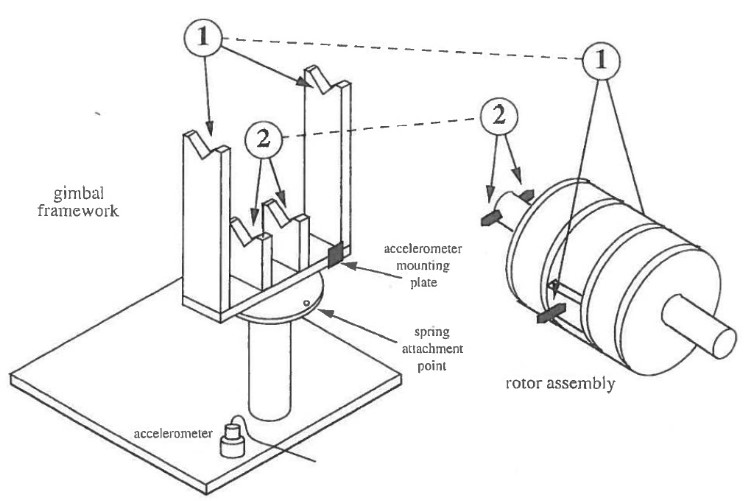
\includegraphics[width=0.5\textwidth]{setup.jpg}
    \caption{Gyroscope assembly}
    \label{fig:setup}
\end{figure}

\section{Theory}

Moment of inertia 

Parallel axis theorem
\begin{equation}
    I_{xx} = I_G + md^2 
\end{equation}

Perpendicular axis theorem
\begin{equation}
    I_{zz} = I_{xx} + I_{yy}
\end{equation}

The dimensions of the rotor can be tabulated as follows:

\begin{table}[H]
    \centering
    \begin{tabular}{|c|c|c|c|}
        \hline
        \multirow{ 2}{*}{Parameter} & \multicolumn{3}{|c|}{Annular Sections} \\
        \cline{2-4}
        & Outer rim & Central Spokes & Inner Rim \\
        \hline
        $r_i$ (mm) & 74 & 26 & 16.5 \\
        $r_o$ (mm) & 85 & 74 & 26 \\
        $L$ (mm) & 63 & 10 & 30 \\
        \hline
        $m$ (kg) & 2.700 & 1.176 & 0.297 \\
        \hline
        $I_{zz}$ (kgm$^2$) & 0.01715	& 0.00362 & 0.00014 \\
        \hline

    \end{tabular}
    \caption{Rotor dimensions}
\end{table}

The mass and moment of inertia of each annulus section is calculated by
\begin{equation}
    m = \frac{\pi}{2} \rho L(r_o^2 - r_i^2), \;\;\;\;\;\; I_{zz} = \frac{\pi}{2} \rho L(r_o^4 - r_i^4)
\end{equation}

These can be added together by parallel axis theorem to give the total moment of inertia of the rotor about the axis of rotation.
Then $C = 2A$ for both the rotor and rotor housing so $I_G = (C + J_1)/2$.
Then the moment of inertia about point 2 as seen in figure \ref{fig:setup} is given by parallel axis theorem as $I_2$.

\begin{alignat}{2}
    \text{Mass of rotor} \;\;\;\; & m \approx 4.173 \text{ kg} \nonumber\\
    \text{Total mass of rotor assembly} \;\;\;\; & M \approx 10.8 \text{ kg} \nonumber\\
    \text{Moment of inertia of rotor about its spin axis, C} \;\;\;\; &  C \approx 0.02091 \text{ kgm}^2 \nonumber \\
    \text{Moment of inertia of rotor assembly, A} \;\;\;\; & I_G \approx 0.08400 \text{ kgm}^2 \nonumber \\
    \text{Moment of inertia of rotor assembly about the rotor axis (excluding rotor)} \;\;\;\; &  J_1 \approx 0.0250 \text{ kgm}^2 \nonumber \\
    \text{Moment of inertia of the gimbal frame about its vertical axis of rotation,} \;\;\;\; &  I_1 \approx 0.0160 \text{ kgm}^2 \nonumber \\
    \text{Spring constant (nominal) of each of the rate gyro springs} \;\;\;\; & k \approx 500 \text{N/m} \nonumber
\end{alignat}

\subsection{Dynamics}

% Euler equations
The Euler equations for an AAC gimble with angular velocity $\bm{\omega}$ in its own reference frame.
The angular velocity of the reference frame is given by $\bm{\Omega}$.
\begin{align}
    A\dot{\Omega}_1 - (A\Omega_3 - C \omega_3) \Omega_2 &= Q_1 \\
    A\dot{\Omega}_2 + (A\Omega_3 - C\omega_3) \Omega_1 &= Q_2 \\
    C\dot{\omega}_3 &= Q_3
\end{align}

In steady precession $Q_1 = Q_3 = 0$, and $\omega_3 >> \Omega_3$.
Using Euler angles in the 
\begin{equation}
    C\omega_3 \Omega_1 = C\omega_3 \dot{\phi} sin \theta = Q
\end{equation}

For nutation neglecting the effects of gimbal inertia, the first and second gyroscope equations can be linearised to give:
\begin{equation}
    \ddot{\omega_1} + \left[ \frac{C\omega_3}{A} \right]^2 \omega_1 = 0 \;\;\;\;\;\;\;\; \ddot{\omega_2} + \left[ \frac{C\omega_3}{A} \right]^2 \omega_2 = 0
\end{equation}
Which both have a frequency of $ p = \frac{C\omega_3}{A} $.

It can be shown that including the effects of gimbal inertia, the nutation frequency is given by
\begin{equation}
    p = \frac{C\omega_3}{A} \left( 1 + \frac{J}{A}cot^2\theta_0 + \frac{I_1}{A}cosec^2\theta_0 \right)
\end{equation}
where $I_1$ is the moment of inertia of the gimbal framework (the stand) about its vertical axis
and $J_1$ is the moment of inertia of the rotor assembly about the rotor axis.

\subsection{Measurement Uncertainty}


\section{Results}

\begin{table}[H]
    \centering
    \begin{tabular}{|c|c|c|c|c|}
        \hline
        Mass (kg) & $Q_{mg}$ (Nm) & Period (s) & $\Omega$ (rad/s) & $Q_{\Omega} $ (Nm) \\
        \hline
        0.5 & 1.03 & 64.72 & 0.09708 & 0.9882898657\\
        1.0 & 2.06 & 33.35 & 0.18840 & 1.917904651\\
        1.5 & 3.09 & 22.03 & 0.28521 & 2.9034099\\
        2.0 & 4.12 & 16.78 & 0.37444 & 3.811806919\\
        \hline
    \end{tabular}
    \caption{Rate of precession with varying mass load at constant $\theta = 90^o$}
\end{table}


\begin{table}[H]
    \centering
    \begin{tabular}{|c|c|c|c|c|}
        \hline
        $\theta$ ($^o$) & $Q_{mg}$ (Nm) & Period (s) & $\Omega$ (rad/s) & $Q_{\Omega} $ (Nm) \\
        \hline
        90 & 4.12 & 16.62 & 0.37805 & 3.848503015\\
        105 & 3.98 & 16.25 & 0.38666 & 3.802010075\\
        120 & 3.57 & 16.47 & 0.38149 & 3.36325567\\
        135 & 2.91 & 15.81 & 0.39742 & 2.860724153\\
        150 & 2.06 & 16.19 & 0.38809 & 1.975358867\\
        \hline
    \end{tabular}
    \caption{Rate of precession with varying $\theta$ at constant mass load $m = 2.0$ kg}
\end{table}

% nutation frequencies
% trial angle meas_freq calc_freq_without_gimbal calc_freq_with_gimbal

% rate Gyro and spring constants

% Cuspidal nutation,
% trial angle period nutations frequency




\section{Discussion}



\section{Conclusion}


\end{document}
